\notocchapter{Additional Plots}
\section{Viscosities of all CESM Experiments}
\label{sec:viscosity-all}
\vfill
\begin{whole}
	\centering\importpgf{figures/appendix/visc-all-x3/}{visc-all-x3.pgf}
\end{whole}
\figcaption{Perpendicular viscosity parameter $B$ for all \grid{x3} runs.\label{fig:viscosity-all-x3}}
\vfill
\clearpage
\null
\vfill
{
	\centering\importpgf{figures/appendix/visc-all-x1/}{visc-all-x1.pgf}\par
}
\figcaption[Perpendicular viscosity parameter \(B\) for all \grid{x1} runs.]{Perpendicular viscosity parameter \(B\) for all \grid{x1} runs. Note the changed scale from \figref{fig:viscosity-all-x3}.\label{fig:viscosity-all-x1}}
\vfill

\notocchapter{An Equatorial Shallow-Water Model (cont.)}
\label{appendix:shallow-water}
The following sections describe some technical aspects of the shallow water model used in \secref{sec:equatorial-shallow-water}. \secref{sec:appendix-sw-implementation} gives a summary of the numerical implementation of the model, while \secref{sec:appendix-sw-verification} focuses on the reproduction of some results found in literature (\cite{killworth} \cite{greatbatch}), in order to verify the consistency of the model, and to allow for the detection of obvious errors in the implementation. Although no quantitative analysis is made, my shallow water model succeeds in reproducing the structure of each solution.

\section{Numerical Implementation}
\label{sec:appendix-sw-implementation}
When implementing numerical models, oceanographers often apply a low-level approach, by explicitly discretizing the model equations using finite differences (see \eg \cite{kaempf}). These implementations are usually very efficient, but on the flip side quite static --- adding additional terms is cumbersome, since the numerical properties of the chosen scheme have to be preserved, and many methods work on regular meshes only.

Because it was important to me that my model supported an \enquote{agile} development style allowing for quick prototyping, I have decided not to implement it from scratch using finite differences, but rather make use of the FiPy software package \citep{fipy}, a finite volume solver framework that is accessed via the Python programming language. FiPy pre-defines finite-volume implementations for the most common terms that appear in \acp{PDE}. On their homepage\sidenote{\url{http://www.ctcms.nist.gov/fipy/}}, the FiPy developers summarize the capabilities of FiPy:

\q{\slshape The solution of coupled sets of PDEs is ubiquitous to the numerical simulation of science problems. Numerous PDE solvers exist, using a variety of languages and numerical approaches. Many are proprietary, expensive and difficult to customize. As a result, scientists spend considerable resources repeatedly developing limited tools for specific problems. Our approach, combining the FV method and Python, provides a tool that is extensible, powerful and freely available. A significant advantage to Python is the existing suite of tools for array calculations, sparse matrices and data rendering.
	
The FiPy framework includes terms for transient diffusion, convection and standard sources, enabling the solution of arbitrary combinations of coupled elliptic, hyperbolic and parabolic PDEs.}

Using FiPy, the actual formulation of the model equations becomes much easier (\listingref{lst:fipy-equations}) and, for the most part, does not depend on the actual numerical implementation of the various terms. This way, I could explore a wide range of problems with different formulations of the model equations and model grids. The FiPy solutions also tended to be quite stable, since most of the terms are solved implicitly\sidenote[-1]{Unfortunately, FiPy does not allow to formulate the shallow-water equations in a fully implicit manner (since the face velocities need to appear as explicit sources).}. However, this comes of course at a computational cost --- by choosing FiPy, I accepted higher run times in exchange for a lower implementation time, which seemed adequate for a project that is as time constrained as a Master's thesis.

\begin{listing}[p]
	\caption[Equation setup for the shallow-water model in FiPy.]{Equation setup for the shallow-water model in FiPy. The cell-centered variables of the model are called \texttt{height}, \texttt{xVelocity}, and \texttt{yVelocity}. Some terms use the rank 1 \texttt{FaceVariable} \texttt{fVelocity}, which is the linearly interpolated velocity at cell faces. \texttt{A} and \texttt{B} are \texttt{CellVariable}s holding the parallel and perpendicular viscosities, respectively. \texttt{WaterSourceBoundary} represents the forcing of the model (Gaussian in the north-western corner of the domain).}
	\label{lst:fipy-equations}
		\begin{listingsbox}{pythoncode}
			diffCoeffX = FaceVariable(mesh=mesh, rank=1)
			diffCoeffX[0] = A.faceValue
			diffCoeffX[1] = B.faceValue
			diffCoeffY = FaceVariable(mesh=mesh, rank=1)
			diffCoeffY[0] = B.faceValue
			diffCoeffY[1] = A.faceValue
			
			fDiv = faceVelocity.divergence
			waterSourceInterior = \
			  (ImplicitSourceTerm(coeff=1.,var=height)-1) / \
			  dampening_scale	 

			xVelocityEq = TransientTerm(var=xVelocity) \
			+ ConvectionTerm(coeff=fVelocity,var=xVelocity) \
			- ImplicitSourceTerm(coeff=fDiv, var=xVelocity) \
			- ImplicitSourceTerm(var=yVelocity,coeff=.5*mesh.y) \
			== \
			- height.grad.dot((1.,0.)) \
			+ DiffusionTerm(diffCoeffX,var=xVelocity)
			
			yVelocityEq = TransientTerm(var=yVelocity) \
			+ ConvectionTerm(coeff=fVelocity,var=yVelocity) \
			- ImplicitSourceTerm(coeff=fDiv, var=yVelocity) \
			+ ImplicitSourceTerm(var=xVelocity,coeff=.5*mesh.y) \
			== \
			- height.grad.dot((0.,1.)) \
			+ DiffusionTerm(diffCoeffY,var=yVelocity)
			
			heightEq = TransientTerm(var=height) \
			+ ConvectionTerm(coeff=fVelocity, var=height) \
			== \
			waterSourceBoundary - waterSourceInterior
			
			# couple equations
			swEquations = xVelocityEq & yVelocityEq & heightEq 
		\end{listingsbox}
\end{listing}

\section{Verification}
\label{sec:appendix-sw-verification}
\subsection{\cite{killworth}}
As%
\sidetable[Parameters used in the first verification run.]{Parameters used in the first verification run. Definitions as in \cite{killworth}.}[tab:killworth-parameters]{%
	\footnotesize%
\begin{align}
	L_x &= \SI{4000}{\kilo\metre}& \\
	L_y &= \SI{2000}{\kilo\metre}& \\
	g &= \SI{0.01}{\metre\per\second\squared}& \\
	\beta &= \SI{2e-11}{\per\second\per\metre}& \\
	H &= \SI{400}{\metre}& \\
	A_h &= \SI{e4}{\metre\squared\per\second}& \\
	Y &= \SI{-75}{\kilo\metre}&
\end{align}
\vspace*{-2\baselineskip}
}[2]%
%
a first step, I have used my shallow-water model to qualitatively reproduce the figures shown in the second part of \cite{killworth}. For this purpose, I have deactivated all forcing (\(\lambda = Q = 0\)), and integrated the model forward for \SI{100}{\day} starting with a dam-break scenario, using parameters as in \tabref{tab:killworth-parameters}\sidenote[-4]{An animation of the adjustment process may be found at \url{https://vimeo.com/145881146}.}, which are the same as used by \citeauthor{killworth}. During the integration, the expected features such as Kelvin waves traveling along the boundaries of the domain are visible.

The final state after \SI{100}{\day} bears a striking resemblance with the corresponding figure from \cite{killworth} (\figref{fig:killworth-comp}). The height field, which coincides with stream lines in high latitudes, shows the same two large circulation cells in the western half of the basin with a comparable magnitude. The velocity field reveals that water predominantly crosses the equator in a western boundary current, from where it either enters the circulation far north, or re-circulates into the southern hemisphere in the interior.

Considering how similar the resulting figures look, given that the two models are implemented using entirely different numerical schemes (finite volume method vs.\ finite differences on a Arakawa C-grid\sidenote[-2]{The Arakawa grids were first introduced by \citet{arakawa}, and are still widely used in geophysical fluid dynamics due to their computational efficiency and conservation properties.}), and presumably use different resolutions (used resolution not reported in \cite{killworth}), I assume my shallow water model to be working correctly for this application.

\begin{figure}
		\subbottom[My model]{%
			\raisebox{.15\totalheight}{\importpgf{figures/appendix/killworth-comp}{killworth-comp.pgf}}%
		}%
		\hfill%
		\subbottom[From \cite{killworth}]{%
			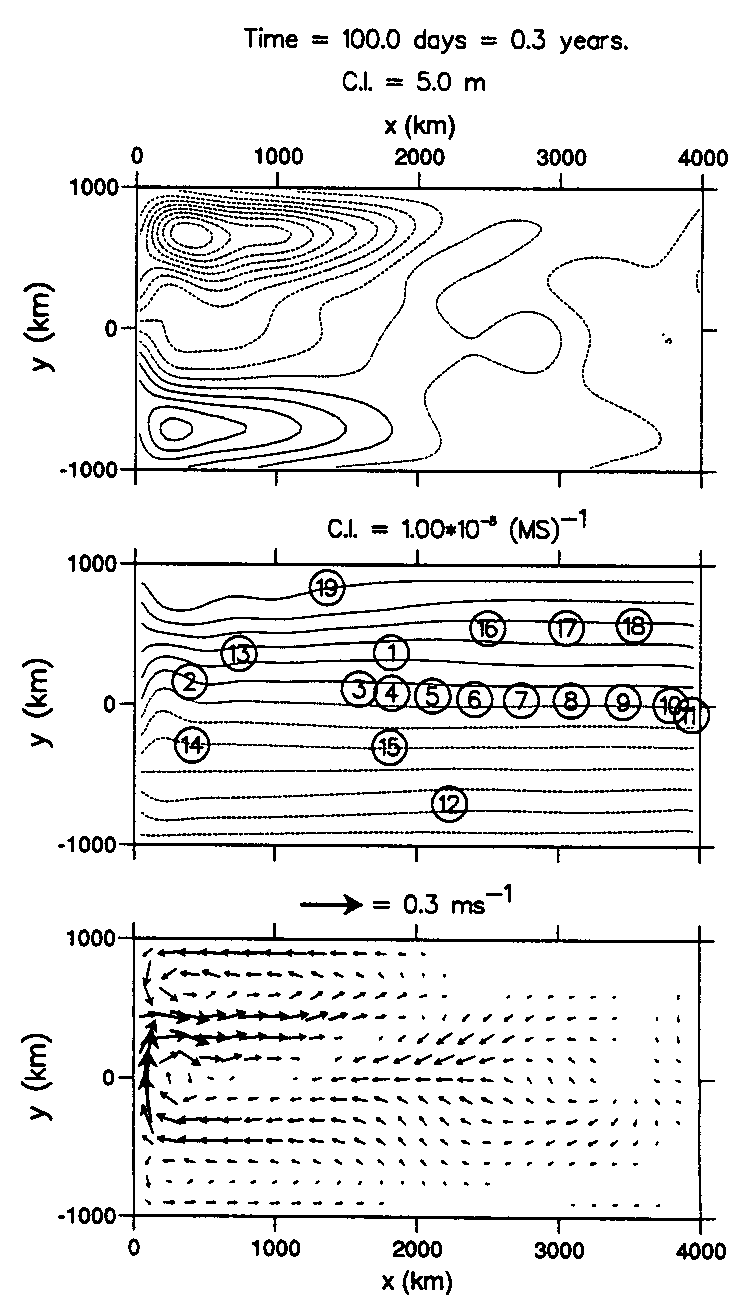
\includegraphics[width=.45\textwidth]{appendix/killworth-sol}%
		}
		\caption[Comparison between a geostrophic adjustment solution from \cite{killworth}, and one created with my own shallow-water model.]{Comparison between a geostrophic adjustment solution from \cite{killworth}, and one created with my own shallow-water model (identical parameters, as in \tabref{tab:killworth-parameters}).}
		\label{fig:killworth-comp}
\end{figure}

\subsection{\cite{greatbatch}}
\cite{greatbatch} contains an interesting study of the \cite{kawase} model, giving a range of numerical solutions for different damping timescales. Since the implementation and used parameters are well described, this publication is a valuable resource to verify my model with a forced reference. However, since the Kawase model equations differ slightly from the ones I have used in my model\sidenote[-3]{\citeauthor{kawase} (and thus \citeauthor{greatbatch}) uses full spherical coordinates, and the \(h\)-equation has been linearized. See also \secref{sec:sw-equations}.}, a comparison has to remain qualitative.

Since we are only interested in the low damping regime\sidenote{Otherwise, deeply penetrating cross-equatorial flow becomes impossible.}, I have used a damping time scale of \SI{1}{\year} for my experiments. Comparing the steady state solution of a high viscosity run with the corresponding figure given in \cite{greatbatch} (\figref{fig:greatbatch-comp}) reveals another striking similarity. In the steady state, the interior height field is symmetric around the equator, with a narrow western boundary current and a wide interior circulation. During spin-up, the same features as described by \citeauthor{greatbatch} can be observed, such as the formation of a swift eastward jet along the equator, that splits up into two branches as a Kelvin wave is emitted by the eastern boundary that arrests the flow at the equator (not shown).

\begin{figure}
		\subbottom[My model]{%
			\raisebox{1.5ex}{\importpgf{figures/appendix/greatbatch-comp}{greatbatch-comp.pgf}}%
		}
		\subbottom[From \cite{greatbatch}]{%
			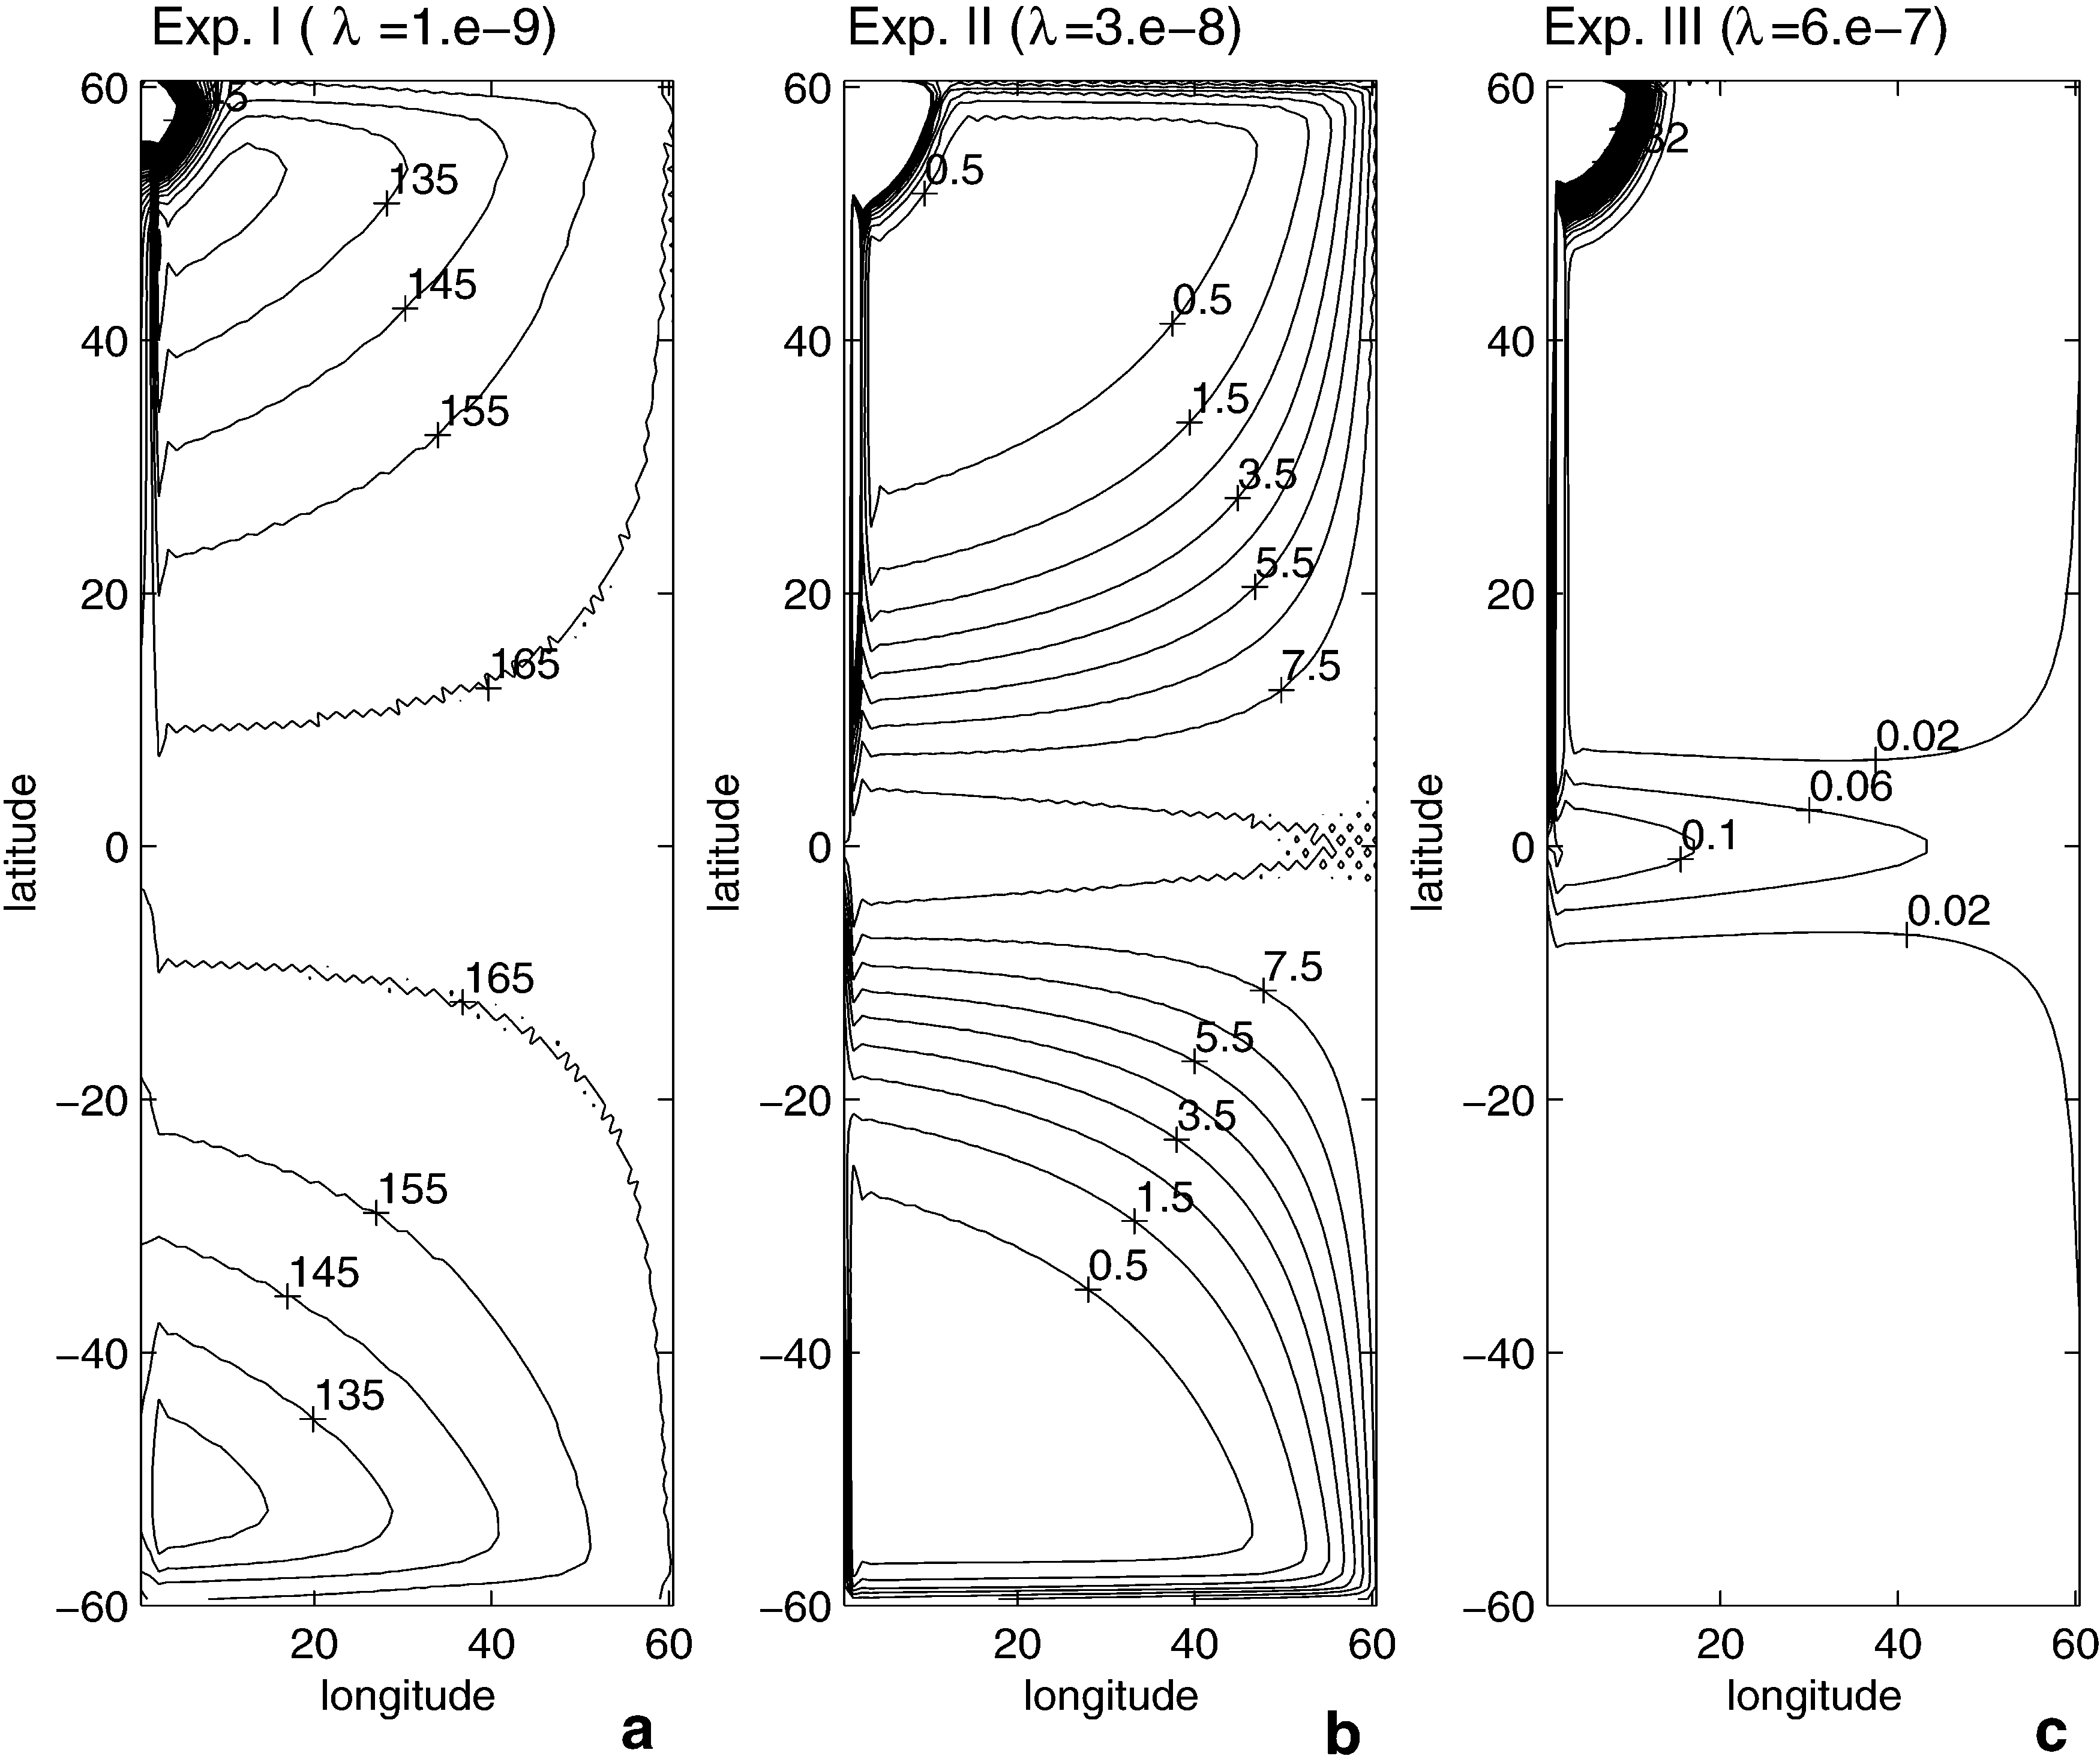
\includegraphics[width=.75\textwidth]{appendix/greatbatch-sol}%
		}
	\caption{Comparison between a steady-state solution from \cite{greatbatch}, and one created with my own shallow-water model.}
	\label{fig:greatbatch-comp}
\end{figure}